\section{quasi-1D}

\begin{comment}
 Outline:

Closed channels, renormalization of conductance *******************
0. Introduction
    a. motivation: why are closed channels important
    b. neglect them
1. Method
    a. numerical simulation model description
        i. generate random scatterer positions
        ii. free space and scatterer matrices multiplied
        iii. self-embedding technique
2. simulation results
    a. for N_c=0, model matches theory
    b. add N_c, there is a deviation in g.
        i. dependence on alpha, density
    c. with scaling, the N_c can be renormalized to N_c=0
        i. recovers lack of dependence on alpha, density
3. why it works
    a. folding technique description
        i. single scatterer
            -eliminate closed channels by matrix element renormalization
        ii. double scatterer
            -adds separation ("density") scaling
    b. supports conclusion on scattering strength alpha, density
4. conclusion
    a. review of main points
       -you can disregard N_c, as long as you do it correctly

Regimes plot development **********************
lengths
boundaries
explanation of regimes, characteristic behavior

Criterion for AL in active random media *****************
various passive criteria comparison


\end{comment}

In quasi-1D, the gain can be put in either the scatterers, the empty medium, or both. If one puts gain in the empty medium, then lasing can occur that is not due to localization (lasing due to boundary conditions of the waveguide). Since we are only interested in lasing due to strong localization, then the gain must be mathematically set in the scatterers. 


Note: our scattering potentials are based on $\delta$ functions, unlike the potentials developed in \cite{2007_Froufe-Perez_PRE} (in Appendix B).


Assume a rectangular metal waveguide with two dimensions, oriented such that the longer dimension is along the z-axis (length), and the shorter direction is the y-axis (width). The rectangular aspect ratio is such that there is no significant propagation along the y-axis (i.e. not two dimensional), but wide enough so that a scatterer does not cause only reflection (which would be one dimensional). Thus we define a quasi-1D waveguide between 1D and 2D. The motivation is to simplify a two-dimensional system using quantization of transverse momentum. This quasi-1D work scales to higher dimensions, unlike true one-dimensional models, which do not have closed channels. Two physical examples of quasi-1D systems are a mesoscopic metal wire and a disordered optical waveguide.

This model permits straightforward generalization to 3D waveguides. However, one would also need to consider the effect of polarization. %?Long-range mesoscopic correlations (?) of fields with different polarization (?)

our quasi-1D model  has the following adjustable parameters: $N_c$, $L$, $\alpha_s$, gain, $W$, $M$, $\omega$, sign of $\alpha_s$. These set the density and $N_o$. For output, we get directly $g$, ${\cal E}$, ${\cal E}^2$, $J_{pw}(z)$, $W_{pw}(z)$, $J_{uf}(z)$, $W_{uf}(z)$, $A(z)$, $B(z)$, $\hat{T}$, $\hat{R}$, correlation of energy(z). From these output, we can get $D(z)$, $\ell_{tmfp}$, $E(y,z)$. 

\subsection{assumptions and abstractions}
\glossary{name={model}, description={a mathematical abstraction of reality, for the purposes of capturing certain phenomena. As such, every model has limitations. }}

For a given model, assumptions must be enumerated.

% meta comment
%when can one be confident that the theoretical model is accurate? Only when the model accurately predicts experimental results

% meta comment
%Models are inherently non-physical because they seek generality. A model is only useful, though, if it captures the desired phenomena (and no extra phenomena). What are the limits of applicability for the models I use?

Specifically, a feature of the quasi-1D waveguide is the delta-function scatterers in free space. This simplifies the math by removing scattering physics, leaving transport physics.

choice of $\delta$-function scatterers has significant consequences:
\begin{itemize}
 \item easier to model mathematically (no spherical scattering math), while retaining the desired phenomenon: scattering from one channel to another
 \item inelastic scattering: no energy loss due to scattering when passive, and phase remains coherent [scatterers only affect amplitude].
 \item non-physical
 \item no saturation limit for number of closed channels
\end{itemize}

No noise is assumed (no spontaneous emission). This means that the transmission with gain will be slightly different compared to real output. Jon's model (from Yale) has noise (1D only).

The gain mechanism is purely mathematical: no atomic level modeling is included. This is part of being mesoscopic regime: independent of atomic conditions.

No input beam properties are assumed, other than the capability to be selectively incident on a specific channel.

By chosing planar quasi-1D geometry (and thus scalar waves), we implicitly assume that polarization will not significantly alter transport phenomena. Although planar geometry may be experimentally realizable, it is not as popular as 3D quasi-1D




\subsubsection{review of channels}

In a waveguide with two dimensions, the wave number $k = \frac{2 \pi}{\lambda} = \frac{\omega}{c}$ is broken into orthogonal components as $k^2 = k_{\parallel}^2 + k_{\bot}^2$. Solving for $k_{\parallel}$,
\begin{equation}
k_{\parallel} = \sqrt{k^2 - k_{\bot}^2}
\end{equation}
where $k_{\bot}$ is defined by the mode number of the sine function perpendicular to the direction of propagation, and is dependent on the waveguide width. %Due to boundary conditions imposed by the metallic (not leaky) waveguide, only wavefunctions that are zero at the boundary will propagate (sine functions in the y direction). Each sine function solution constitutes a ``channel.''
The two components are thus
\begin{equation}
 \begin{gathered}
  k_{\bot_n} =  \frac{n \pi}{W} \\
  k_{\parallel_n} = \sqrt{\left( \frac{2 \pi}{\lambda} \right)^2 - \left(\frac{n \pi}{W}\right)^2}
 \end{gathered}
\label{eq:wave_number_quasi1d}
\end{equation}
Note that for sufficient channel index, $k_{\parallel}$ becomes imaginary, denoted $i \kappa_{\parallel}$.  These channels, with an imaginary wave number, are the evanescent channels. The intensity decays exponentially because the exponent is real ($e^{i(i\kappa x)}$). 
% NOTE: Vellekoop's thesis says this is equivalent to spacial distribution (speckle) but gives no math


%%%%%%%%%%%%%%%%%%%%%%%%%%%%%%%%%%%%%%%%%%%%%%%%%%%%%%%%%%%%%%%%%%%%%%%%%%%%%%
\subsection {Introduction}
%%%%%%%%%%%%%%%%%%%%%%%%%%%%%%%%%%%%%%%%%%%%%%%%%%%%%%%%%%%%%%%%%%%%%%%%%%%%%%

In experimental studies of quasi-1D systems with randomly positioned 
scatterers there are open (propagating) channels and closed (evanescent)
channels.  
Dorokhov-Mello-Pereyra-Kumar (DMPK) theory 
%\cite{1988_Mello_Kumar_DMPK} 
%\cite{1982_Dorokhov_DMPK}
for quasi-1D geometry assumes
(1) all open channels are the same, and (2) closed channels can be disregarded.

Since the closed channels decay exponentially one normally
neglects these contributions in numerical simulations. If the detector is far way from the media
then the closed channels won't contribute. 

This is desirable, as the math is easier 
(which translates computationally to faster), and it is justified analytically
by calculations done for single scatterers~\cite{1990_Bagwell}~\cite{1991_Kumar_Bagwell}
and by rationalizing that if the density of scatterers is low enough, then 
there is sufficient separation between scatterers that closed channels do 
not contribute to interaction. However, since we are interested in Anderson 
localization, we will be in the high density, low scattering strength regime.
In this regime it would appear that we can not ignore the effect
of closed channels.  Then the ability to numerically model systems becomes
questionable since real systems have an infinite number of closed channels.

A numerical simulation is described that models an arbitrary number of point scatterers
in a quasi-1D waveguide where each has the same scattering strength. 
We can vary the number of open and closed channels,
scattering strength, system dimensions, and scatterer density. 
The significance of closed modes can be studied through 
numerical simulation to determine how a finite number of these modes 
affect the wave propagation through the random medium.  In a real 
system there are an infinite number of closed channels.  It is
shown that closed channels can be ignored, which is useful as accounting for an infinite
number is difficult or impossible.
Using this computational model we verify theoretical concepts. Self-embedding 
technique
%~\cite{1999_yamilov_selfembed}
~\cite{1976_Bellman_Wing_embedding}
extends the limits of numerical simulation when closed channels are added, but this
does not allow for an arbitrary number of closed channels as numerical inaccuracy
still emerges.

The scattering matrices for one scatterer and two scatterers are also
derived. We show that folding the closed channels is both possible, and in numerical 
simulation, necessary.  

This work applies to higher dimensions in that it scales, unlike one-dimensional
models which do not have closed channels. Physical examples of quasi-1D systems 
are mesoscopic metal wire and disordered optical waveguide.

Conductance g is observed to be uniform, even if contribution of the channels
are non-uniform [need more here]. 

\begin{equation}
g = \sum_a \sum_b T_{a,b}
% See Ben's notes, 20080610
\end{equation}

Scattering length as a function of three parameters, density, scattering strength, and number of closed, or 
evanescent, channels is determined. (?)

Quantization of transverse momentum allows for the simplification of 
this two-dimensional system to a one-dimensional system referred to as 
quasi-1D. This model permits straightforward generalization to 3D waveguides, 
in which one would need to consider the effect of polarization, such as long-range mesoscopic 
correlations (?) of fields with different polarization.

%%%%%%%%%%%%%%%%%%%%%%%%%%%%%%%%%%%%%%%%%%%%%%%%%%%%%%%%%%%%%%%%%%%%%%%%%%%%%%
\subsubsection {Numerical Simulation Model Description}
%%%%%%%%%%%%%%%%%%%%%%%%%%%%%%%%%%%%%%%%%%%%%%%%%%%%%%%%%%%%%%%%%%%%%%%%%%%%%%

Evolution of electric field through the system is 
described with a set of transfer matrices in terms of open and closed channels
of the waveguide.  This ensures the continuity of both the electric field 
and its derivative throughout the waveguide.  Parameters such as the length
and width of the waveguide, the number of open and closed channels (real 
and evanescent modes), the number of scatterers, and the scattering strength
of scatterers determine how the light will propagate through the 
waveguide. The wave vector k for both open and closed channels is calculated,
n being the mode number, W the width, c speed of light in a vacuum.

\begin{equation}
\begin{gathered}
k_{\perp n}=n\pi /W \\
k_{\parallel n}=\sqrt{(w/c)^2-k_{\perp n}^2}
\end{gathered}
\label{kwaveguide}
\end{equation}

The wavelength is normalized to one for all simulations.  
% Maybe not?: 
%[wavelength] lambda * [frequency] f = [angular frequency] omega / [wavenumber] k
Each channel, open and closed, has both a perpendicular and parallel wave vector components.
From Equ.~\ref{kwaveguide} if $K_{\parallel n}$ is real the channel is open, $K_{\parallel n}$ imaginary 
corresponds to closed.  The total number of channels ($N_{max}$) is
studied systematically to determine the effects of closed channels and 
includes the open channels.

Wave propagation is described as follows.  The values for the electric 
field and its derivative are stored for each mode at each layer, scatterer 
or free space, in matrices. The electric field and its derivative for free 
space propagation of open channels are given by:

\begin{equation}
\begin{gathered}
E_n(x+\Delta x)=E_n(x)cos(K_{\parallel n}\Delta x)+K_{\parallel n}^{-1}
E_n^{'}(x)sin(K_{\parallel n}\Delta x) \\
K_{\parallel n}^{-1}E_n^{'}(x+\Delta x)=-E_n(x)sin(K_{\parallel n} \Delta x)
+K_{\parallel n}^{-1}E_n^{'}(x)cos(K_{\parallel n}\Delta x)
\end{gathered}
\label{electricfield}
\end{equation}

For the closed channels, the field equations are the similar to 
Equ.~\ref{electricfield} except $K$ is replaced by the imaginary $\kappa$.

\begin{comment}
%% REDUNDANT
\begin{equation}
\begin{gathered}
E_n(x+\Delta x)=E_n(x)cosh(\kappa_{\parallel n}\Delta x)+
\kappa_{\parallel n}^{-1}E_n^{'}(x)sinh(\kappa_{\parallel n}\Delta x)\\
\kappa_{\parallel n}^{-1}E_n^{'}(x+\Delta x)=E_n(x)sinh(\kappa_{\parallel n}
\Delta x)+\kappa_{\parallel n}^{-1}E_n^{'}(x)cos(\kappa_{\parallel n}\Delta x)
\end{gathered}
\end{equation}
\end{comment}

The electric field after each scattering event must be equal to the
initial field, where the first derivative is given by:

\begin{equation}
\begin{gathered}
E_n(x+\Delta x)=E_n(x)\\
E_n^{'}(x+\Delta x)=E_n^{'}(x)-\alpha(\frac{\omega}{c})^2\sum_{m=1}^{n_{max}}
A_{nm}E_m(x) 
\end{gathered}
\end{equation}

and

\begin{equation}
A_{nm}=\frac{2}{W}sin(K_{\perp n}y)sin(K_{\perp m}y)
\end{equation}
\begin{equation}
K_{\parallel n}=i\kappa_{\parallel n}
\end{equation}

Alpha describes the scattering strength of the scatterers. Thus wave
propagation can be described by $2 N_{max} x 2 N_{max}$ matrices of two types:
propagation or free space matrices, and scattering matrices. 
See Fig.~\ref{fig:tomsmatrices}

\begin{figure}
\vskip -0.5cm
\centerline{
\scalebox{1}{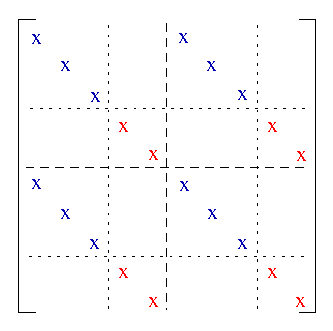
\includegraphics{pictures/propagation_matrix}}
\quad \quad \quad \quad
\scalebox{1}{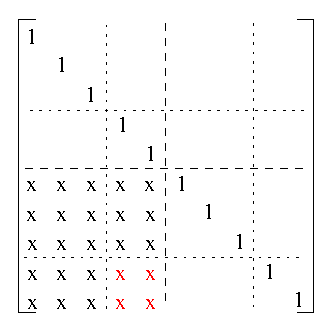
\includegraphics{pictures/scattering_matrix}}}
\vskip -0.5cm
\caption{Propagation or Free Space Matrices (left),
and Scattering Matrices (right). ``x'' denotes non-zero terms, which are not necessarily the same. 
Each matrix is separated into four $N_{max} x N_{max}$ quadrants 
(long dashed portions), each containing information from open channels
(upper left short dashed portions) as well as closed (lower right short
dashed portions). }
\label{fig:tomsmatrices}
\end{figure}

These matrices are combined to form a total matrix.
This matrix contains the propagation of the CW electric field information through the 
waveguide. The total matrix is used to calculate the reflection and
transmission coefficients for each mode.

%%%%%%%%%%%%%%%%%%%%%%%%%%%%%%%%%%%%%%%%%%%%%%%%%%%%%%%%%%%%%%%%%%%%%%%%%%%%%%
\subsubsection {Self-Embedding}
%%%%%%%%%%%%%%%%%%%%%%%%%%%%%%%%%%%%%%%%%%%%%%%%%%%%%%%%%%%%%%%%%%%%%%%%%%%%%%

Due to the numerical instability which builds up in longer disordered
waveguides, the computation of the simple product of individual matrices is
not sufficient, as the eignvalues become divergent. The self-embedding method is introduced 
slow the growth of computational error inherent in numerical matrix multiplication.
This method consistently corrects any deviation caused by rounding on every step of the multiplication and 
gives increased accuracy to the final result.  % I don't think this is correct; it just prolongs the time until matrices become unstable (determinant not equal to 1)

Start with the vector describing $N$ open and $N_c$ closed channels for both
the electric field and the field derivative, total length $N+N_c+N+N_c$, on the
incident side of the medium: $\vec{v}(0)$.  There is a similar vector on the otherside
of the quasi-1D waveguide, $\vec{v}(L)$, of the same dimension. For $\vec{v}(0)$, assume a an
input beam in one channel, $n_0$. (Later on the input channel will be iterated over
all open channels. The input could be to closed channels, but that is not investigated
in this letter.)

Given $\vec{v}(0)$ and $\vec{v}(L)$ a pair of matrices is sought that satisfies
\begin{equation}
\hat{G}\vec{v}(0) + \hat{H}\vec{v}(L) = \vec{v}_{BC}
\label{selfEmbedGHvBC}
\end{equation}
such that $\vec{v}_{BC}$ has no dependence on variables, transmission, or reflection.
Any $\hat{G}$ and $\hat{H}$ that satisfies these conditions can be used. We use
Fig.~\ref{fig:HGmatrix} which results in $\vec{v}_{BC}$ having zeros in all elements
except for the input channel, where there is a ``2''.  

Now that $\hat{G}$ and $\hat{H}$ are set, S is

\begin{equation}
\hat{S} = (\hat{H} + \hat{G})^{-1}
\label{selfEmbedSinvGH}
\end{equation}



Self-embedding uses inverses, which add to computational time.


%~\cite{1999_yamilov_selfembed}
%~\cite{1976_Bellman_Wing_embedding}

\begin{figure}
\vskip -0.5cm
\centerline{
\scalebox{1}{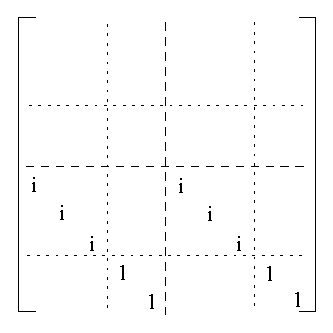
\includegraphics{pictures/H_matrix}}
\quad \quad \quad \quad
\scalebox{1}{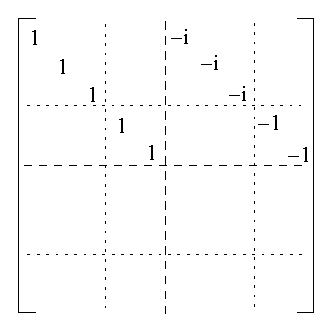
\includegraphics{pictures/G_matrix}}}
\vskip -0.5cm
\caption{Boundary conditions (?). H on left, G on right.}
\label{fig:HGmatrix}
\end{figure}

Transmission and reflection vectors are related to the S matrix
(part of the total matrix(?)) that is determined via the self-embedding procedure:

Each time the simulation self-embeds multiple matrix inversions must
be calculated (?).  These calculations take longer than a simple matrix
multiplication, but the method prevents the buildup of numerical
error (describe this more).  More self-embedding loops means a longer simulation run time.

Even with self-embedding technique, the number of closed channels is computationally limited.
The numerical limits depend on scattering density, system length (number of transfer matrices).

%%%%%%%%%%%%%%%%%%%%%%%%%%%%%%%%%%%%%%%%%%%%%%%%%%%%%%%%%%%%%%%%%%%%%%%%%%%%%%
\subsection {Numerical simulation results}
%%%%%%%%%%%%%%%%%%%%%%%%%%%%%%%%%%%%%%%%%%%%%%%%%%%%%%%%%%%%%%%%%%%%%%%%%%%%%%
%
%outline:
%    a. for N_c=0, model matches theory
%    b. add N_c, there is a deviation in g.
%        i. dependence on alpha, density
%    c. with scaling, the N_c can be renoralized to N_c=0
%        i. recovers lack of dependence on alpha, density

This table shows the preliminary results of the scattering lengths
obtained using this method.  The scattering lengths describe the rate at which
the energy is removed from the input channel.  It is a function of two
parameters, the scattering density and the strength of the individual
scatterer.  The results displayed on the following page show, as expected,
the scattering lengths decrease as the scattering strength increases.  This is
also the trend for density.

\begin{figure}
\vskip -0.5cm
\centerline{
\scalebox{.5}{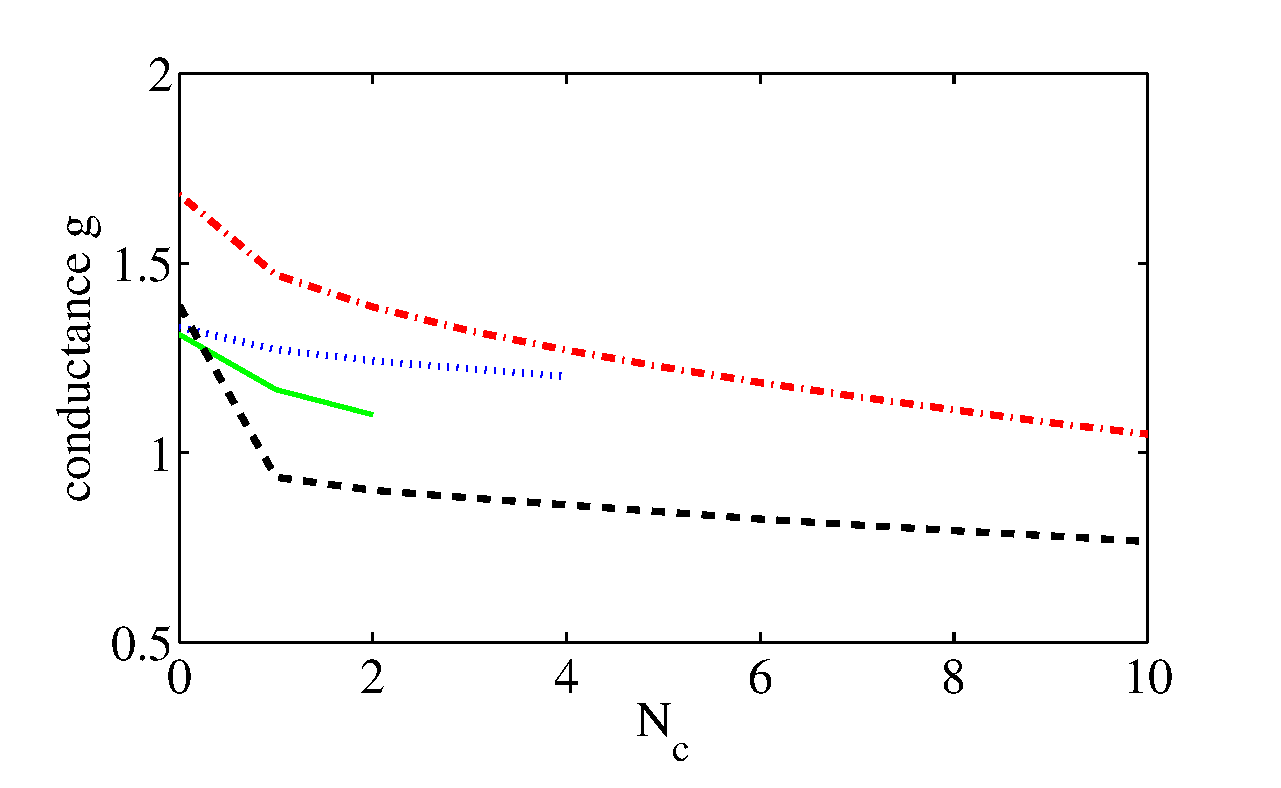
\includegraphics{pictures/conductivity_g_versus_N_closed}}}
\vskip -0.5cm
\caption{conductance versus number of closed channels $N_c$ for varying
scattering strength and density. (Which is which?) Dotted blue is, solid
green is, dot-dashed red is, and dashed black is .}
\label{fig:gVersusNc}
\end{figure}
  %Supporting charts or tables that demonstrate the scattering length
  %dependence on density and alpha

The figures above illustrate the transition which occurs in the transmission
matrix ($T_{ab}$) as the length of the sample increases for a fixed density and
scattering strength.  A is the input channel number (Horizontal axis) and B is
the output channel number (Vertical axis).  One can see initially that the
shortest sample (left) only the diagonal components of not equal to zero.
This corresponds to the wave emerging from the same channel as it was launched
into.  One can see from the right panel, for a very long system, the light
emerges in all output channels.

\begin{figure}
\vskip -0.5cm
\centerline{
\scalebox{.3}{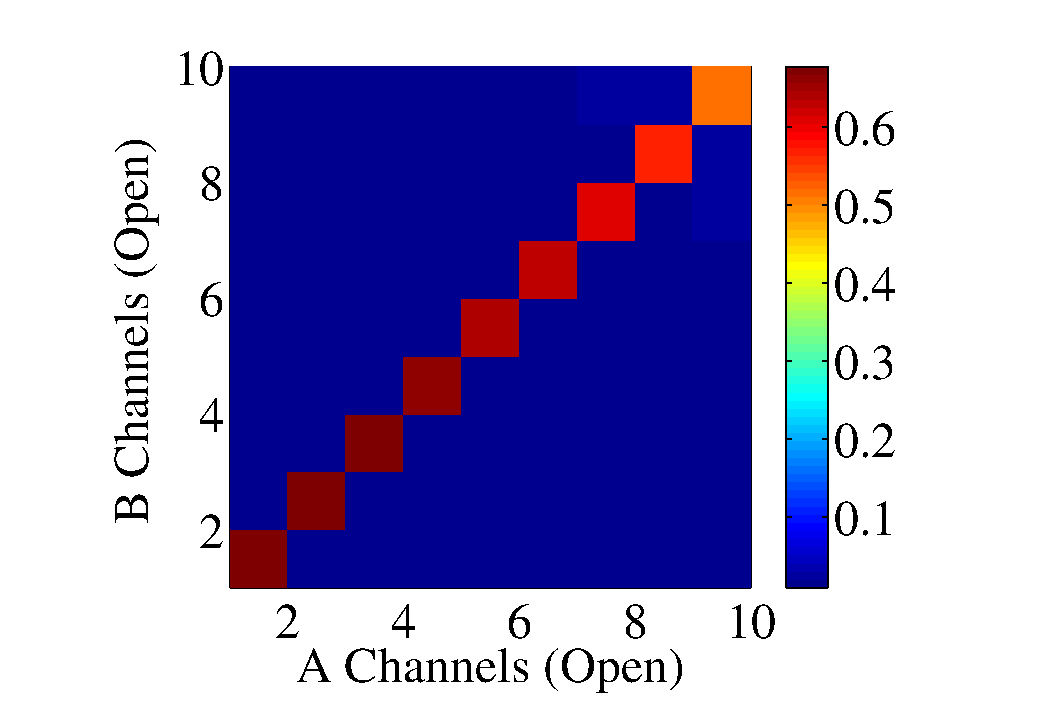
\includegraphics{pictures/low_scattering}}
\scalebox{.3}{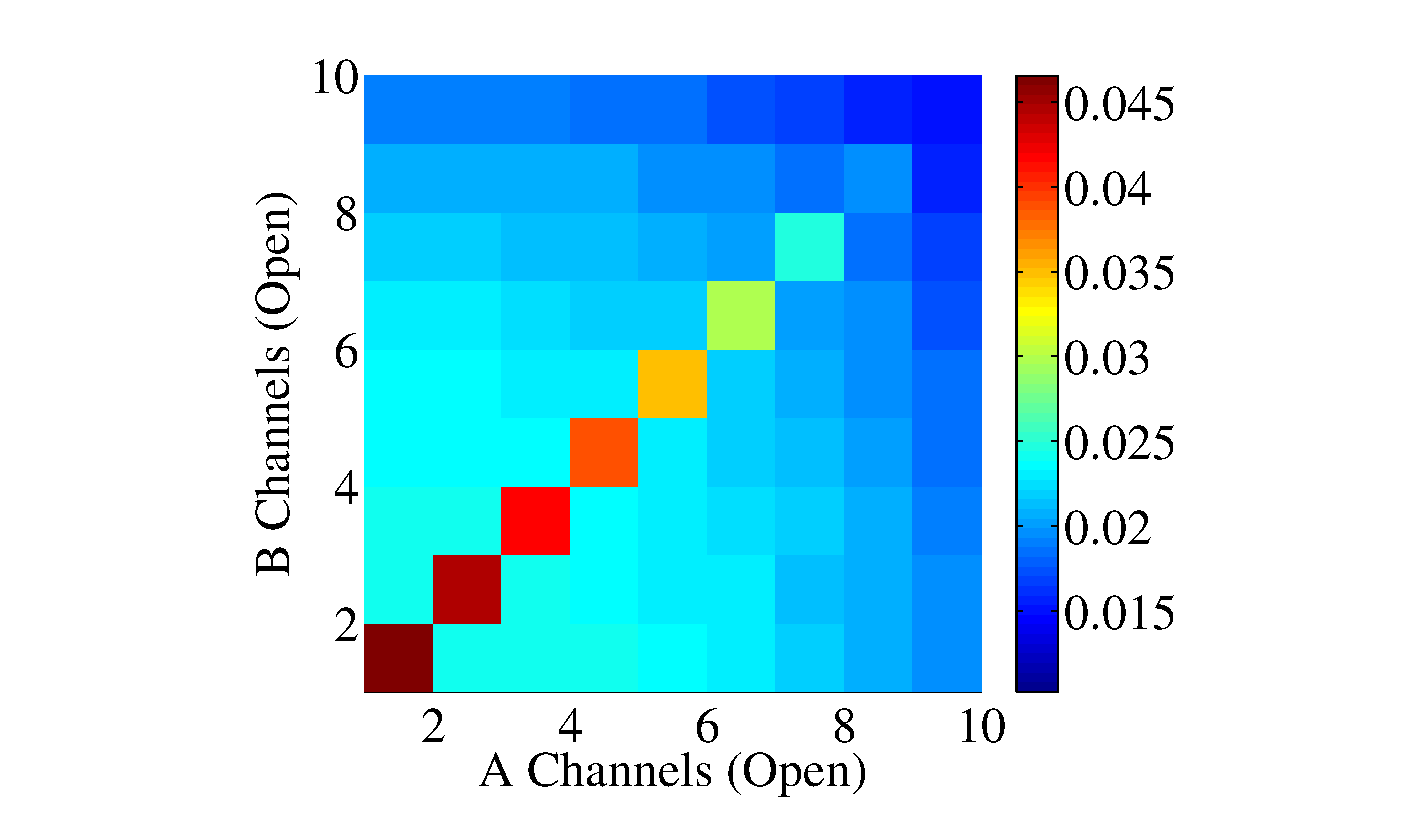
\includegraphics{pictures/mid_scattering}}
\scalebox{.25}{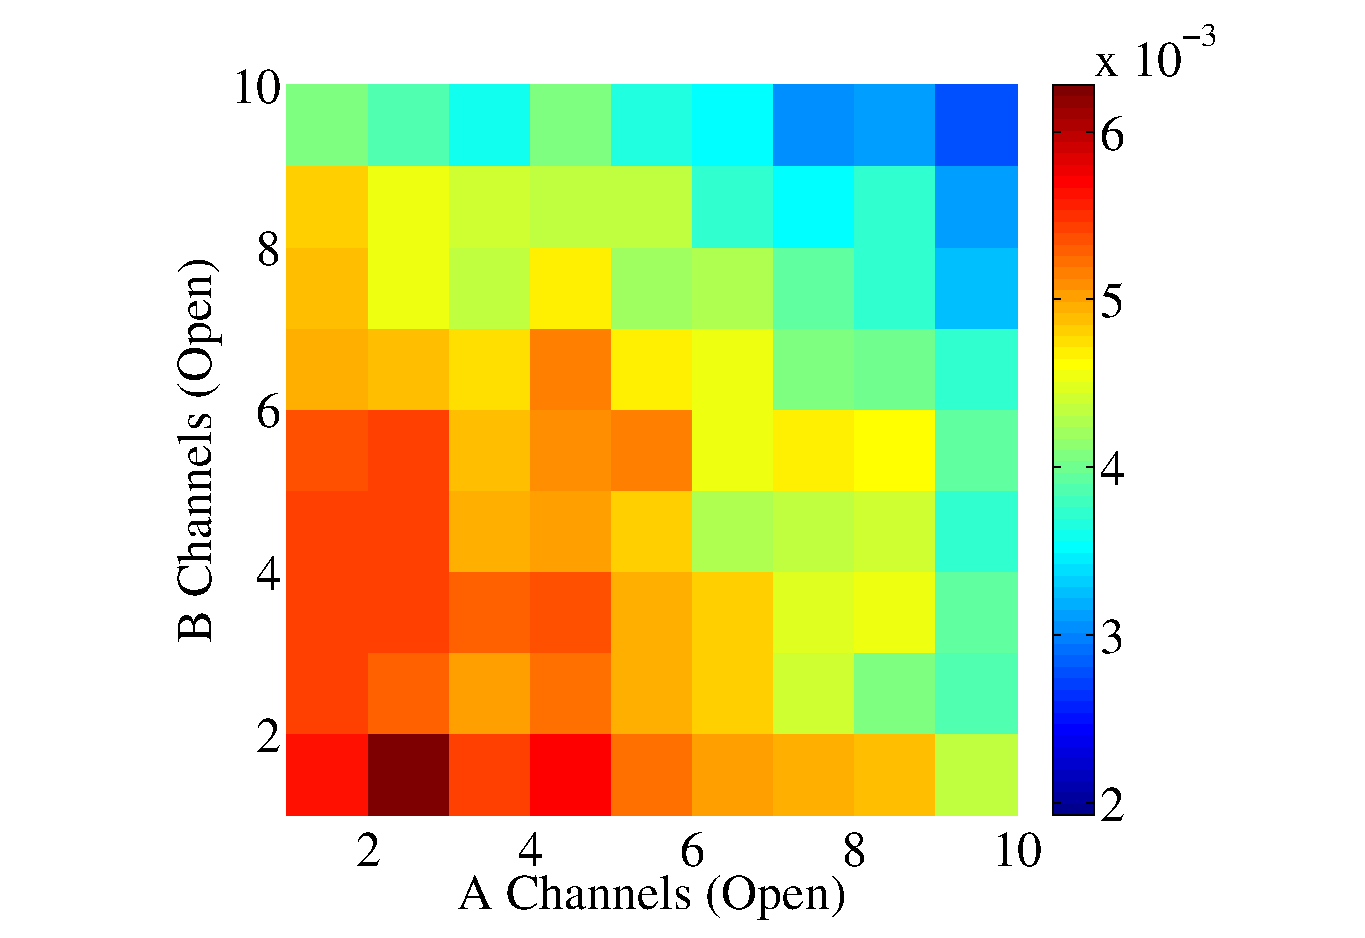
\includegraphics{pictures/high_scattering}}}
\vskip -0.5cm
\caption{Matrices describing scattering from an input channel to an output channel
for 10 open channels; arbitrary units?  Left: for few scattering events in the 
medium it is likely that light will not scattering into a different channel. Even
at low scattering probability the channels are not uniform (higher concentration
of (?) in lower channel numbers). As the scattering event probability is increased
(higher scatterer density or longer system length), inter-channel scattering is 
observed.  At high scattering density (?)}
\label{fig:channelMatrices}
\end{figure}


The model suggests that saturation (a finite number of closed 
channels) is attainable given that the parameters fit a constraint:
\begin{equation}
(m / (\hbar^2 \kappa _n))(\lambda/W) <<1
\end{equation}
% page 358 of \cite{1990_Bagwell}



%%%%%%%%%%%%%%%%%%%%%%%%%%%%%%%%%%%%%%%%%%%%%%%%%%%%%%%%%%%%%%%%%%%%%%%%%%%%%%
\subsection {Why closed channels can be renormalized: Quasi-1D theoretical models}
%%%%%%%%%%%%%%%%%%%%%%%%%%%%%%%%%%%%%%%%%%%%%%%%%%%%%%%%%%%%%%%%%%%%%%%%%%%%%%
%    a. folding technique description
%        i. single scatterer
%            -eliminate closed channels by matrix element renormalization
%        ii. double scatterer
%            -adds seperation ("density") scaling
%    b. supports conclusion on scattering strength alpha, density

In order to model quasi-1D system with random defects one must know how to 
deal with a single defect. It is then assumed that additional defects can be
extrapolated. The math for a single defect in a waveguide can be dealt with 
using transfer matrices or Greene's functions %~\cite{??}.

A matrix that describes open and closed channels is of size $(N+N_c)x(N+N_c)$
where $N$ is the number of open channels, $N_c$ is the number of closed channels.
We derive in appendix A how to reduce matrices of rank $N_c$ to rank $N$,
called folding, as the closed channels are incorperated into the open channels.
There is a conservation of information, in that the information stored in the original
$(N+N_c)x(N+N_c)$ matrix is still contained within the new ``folded'' $NxN$
matrix, albeit messier elements.  Although messier, by
induction (using the developed recursion relation) it has been demonstrated that 
an $NxN$ matrix can account for N open channels and an infinite number of closed channels $N_c$.  The math
done is a correction to ~\cite{1990_Bagwell} and is a more explicit reworking of~\cite{1991_Kumar_Bagwell}.

With a single scatterer model scattering strength can be modeled, 
but the separation between two scatterers is not present. Thus if 
there are many scatterers the effect of density on scattering length can not
be accounted for by a single scatterer. In order to model interaction of 
scatters by both the open and closed channels, one needs to derive the math
for at minimum two scatterers, as is done in %~\cite{??}.

%%%%%%%%%%%%%%%%%%%%%%%%%%%%%%%%%%%%%%%%%%%%%%%%%%%%%%%%%%%%%%%%%%%%%%%%%%%%%%
\subsection {Conclusion}
%%%%%%%%%%%%%%%%%%%%%%%%%%%%%%%%%%%%%%%%%%%%%%%%%%%%%%%%%%%%%%%%%%%%%%%%%%%%%%
% outline:
% i structure of the model
% divergence of closed channels
% Nc is important to include but hard to model (due to divergence)
% conclusion: can ignore Nc, but need to renormalize mean free path
% include a discussion of self-embedding
% why self-embedding necessary:
% 	exponential behavior of closed channels
% 	open and closed channels cause divergence in matrices
% 	 -> self-embedding renormalizes the matrices and reduces the divergence

Using a numerical simulation of a quasi-1D waveguide with densely packed
randomly placed scatterers the effect of closed channels on was investigated.
Using transfer matrices, open and closed channels are varied.  The number of
matrices multiplied is limited by numerical accuracy, and is extended using self-embedding technique.

However, even with a perfect numerical simulation the effect of closed channels
can not be accounted for, as (?) does not reach an asymptote.

Thus analytically folding the closed channels is necessary.  The effect on 
numerical simulations is acceptable by renormalizing conductance.

Verified that the numerical model, analytical single scatterer, and 
analytical two scatterer results match.


Increasing $N_c$ is effectively the same as increasing system Length. Thus we can 
disregard $N_c$ (?) Or maybe this is a way to account for it?

The folding (in the appendix) shows that one can disregard $N_c$ by using a 
different NxN matrix

